% Stage 3 report, revision 5: v4 with the review comments applied (recap rewritten, ltp moved to
% Stage 4, EV6 and 10x-leakage experiments dropped, figures 3 and 5 regenerated).
% Compile from this folder: pdflatex stage3_v5.tex (twice).
\documentclass[11pt,a4paper]{article}
\usepackage[margin=2.2cm]{geometry}
\usepackage[T1]{fontenc}
\usepackage{lmodern}
\usepackage{amsmath}
\usepackage{graphicx}
\usepackage{booktabs}
\usepackage{array}
\usepackage{enumitem}
\usepackage{xcolor}
\usepackage{caption}
\usepackage{float}
\usepackage[section]{placeins}
\usepackage[hidelinks]{hyperref}
\graphicspath{{../experiments/}}
\setlist{itemsep=1pt,topsep=3pt}
\setlength{\parindent}{0pt}
\setlength{\parskip}{4pt}
\captionsetup{font=small,labelfont=bf}
\newcommand{\us}{\,$\mu$s}
\newcommand{\degC}{\,\textdegree C}

\begin{document}

\begin{center}
{\LARGE\bfseries Lightweight Temperature Predictor:}\\[4pt]
{\Large\bfseries TapaSense}\\[4pt]
{\large Stage 3 Report}\\[8pt]
Ethan Bobby Kurien \quad Kaivalya Mase
\end{center}

%=====================================================================
\section{Work so far: the steady-state model}\label{sec:recap}
TapaSense predicts the temperature of every core of a multi-core chip from the core powers,
matching the HotSpot simulator~\cite{hotspot} to within 0.5\,K on average and 1\,K at worst, in
microseconds and a few kilobytes. Stages 1--2 built and validated the steady-state model S1; this
stage adds a transient model, so that temperatures can be followed over time.

\textbf{S1, the influence matrix.} The steady temperature of every block of the floorplan is
\begin{equation}
  T = T_\text{amb} + G\,P,
  \label{eq:s1}
\end{equation}
where $P$ is the vector of core powers (W), $T_\text{amb}$ the ambient temperature, and $G$ the
\emph{influence matrix}: $G_{ij}$ is the steady temperature rise of block $i$ (K) per watt in core
$j$. Column $j$ of $G$ is measured directly by one steady HotSpot run with 1\,W in core $j$, so
8 runs (about 4\,s) calibrate a floorplan.
\begin{itemize}
  \item \textbf{Exact.} S1 reproduces HotSpot to its 6-decimal output (0.00003\,K worst on 7{,}248
        test runs) and always picks the right hottest core.
  \item \textbf{Cheap.} One matrix--vector product per prediction (2.6\us) and 928\,B per
        floorplan (464\,B in 32-bit numbers).
  \item \textbf{Calibration is needed.} Every calibration-free alternative (a generic heat-spread
        kernel, or $G$ borrowed from another floorplan or predicted from geometry) was 0.5--2.7\,K
        off on average and up to 12\,K.
\end{itemize}

\textbf{Floorplans.} The main set is 24 floorplans: the 23 given ones and HET-A, our own
heterogeneous layout. Each has $N = 8$ cores (2 big, 6 little).

%=====================================================================
\section{Transient models}\label{sec:models}

\subsection{Calibration data: step responses}\label{sec:steps}
Because HotSpot is linear, its temperature response to any power trace is \emph{fixed by the
response to a 1\,W step in each core}. Transient calibration therefore records these step
responses: $s_{ij}(t)$ is the temperature rise of core $i$ at time $t$ after 1\,W is switched on in
core $j$.

\subsection{T1: one time constant (baseline)}
The simplest transient model lets each core move a fixed fraction of the way towards its S1
steady value at every time step:
\begin{equation}
  x_i[k+1] = a_i\, x_i[k] + (1 - a_i)\,(G\,P[k])_i, \qquad a_i = e^{-\Delta t/\tau_i},
  \qquad T_i = T_\text{amb} + x_i,
  \label{eq:t1}
\end{equation}
where $x_i$ is core $i$'s temperature rise above ambient, $\Delta t$ the time step at which the
model predicts (1\,ms), and $\tau_i$ one time constant per core, fitted so that the model's step
response $G_{ij}(1 - e^{-t/\tau_i})$ is as close as possible to the measured $s_{ij}(t)$.

\subsection{T2: ARX, calibrated from one long trace}\label{sec:arx}
Instead of step responses, ARX is fitted to one long recorded HotSpot trace. ARX (\emph{autoregressive with exogenous input}) predicts the
next temperature from its own past values and from an outside input, here the power. It is the
standard way to
model a system from recorded inputs and outputs alone, and similar models have predicted
temperature from past temperatures~\cite{coskun09} or from measured power and
temperature~\cite{singla15}.

\textbf{Calibration trace.} 60\,s at 1\,ms steps, from a cold chip.
Every core switches independently between random power levels, with phases of 1\,ms to 5\,s, so
both fast and slow behaviour is excited.

\textbf{The model.} The next temperature rise above ambient is a weighted mix of the last few rises
and powers. With $n_a$ past rises and $n_b$ powers, written ARX$(n_a, n_b)$:
\begin{equation}
  x[k] = \sum_{l=1}^{n_a} A_l\, x[k-l] + \sum_{l=0}^{n_b-1} B_l\, P[k-l],
  \label{eq:arx}
\end{equation}
where $A_l$ and $B_l$ are matrices of coefficients; for example $x[k] = A_1 x[k-1] + A_2 x[k-2] + B_0 P[k] + B_1 P[k-1]$ for ARX(2,2).

\subsection{T3: sum of exponentials}\label{sec:t3}
The step response $s_{ij}(t)$ says how core $i$ heats up, over time, after 1\,W is switched on in
core $j$: it starts at 0 and ends at the steady value $G_{ij}$. T3 writes it as a sum of $M$ rising
curves:
\begin{equation}
  s_{ij}(t) \approx \sum_{m=1}^{M} a_{ijm}\left(1 - e^{-t/\tau_m}\right),
  \qquad \sum_m a_{ijm} = G_{ij}.
  \label{eq:t3}
\end{equation}
The curves, set by the time constants $\tau_m$, are the same for every pair of cores; only the
weights $a_{ijm}$ differ, and they say how much of the heating of core $i$ by core $j$ happens at
each speed. The weights of each pair add up to $G_{ij}$, so T3 ends at exactly S1's value: it is
exact in steady state.

%=====================================================================
\section{Results}\label{sec:results}

\subsection{Fit to the step responses (calibration data)}
This is how closely each model reproduces the step runs it was calibrated on; the error is the
largest difference from HotSpot over the response to switching on the nominal power of all cores
(20\,W per big core and 8\,W per little core, 88\,W in total). Errors on unseen test traces follow
in Section~\ref{sec:follow}. The six time constants fitted with $M = 6$ are about 1\,ms, 3\,ms,
26\,ms, 89\,ms, 0.56\,s and 8.1\,s.

\begin{center}
\small
\begin{tabular}{@{}l c c@{}}
\toprule
Model & Worst fit error, main set (24 floorplans) & Size \\
\midrule
T1 (one time constant per core) & 14.1\,K & 1.0\,kB \\
T3, $M=2$ & 2.82\,K & 1.9\,kB \\
T3, $M=3$ & 1.04\,K & 2.8\,kB \\
T3, $M=4$ & 0.46\,K & 3.7\,kB \\
T3, $M=6$ & 0.12\,K & 5.6\,kB \\
\bottomrule
\end{tabular}
\end{center}
One time constant (T1) cannot follow a response spanning 1\,ms to 8\,s. T3 converges quickly with
$M$.

\begin{figure}[H]
  \centering
  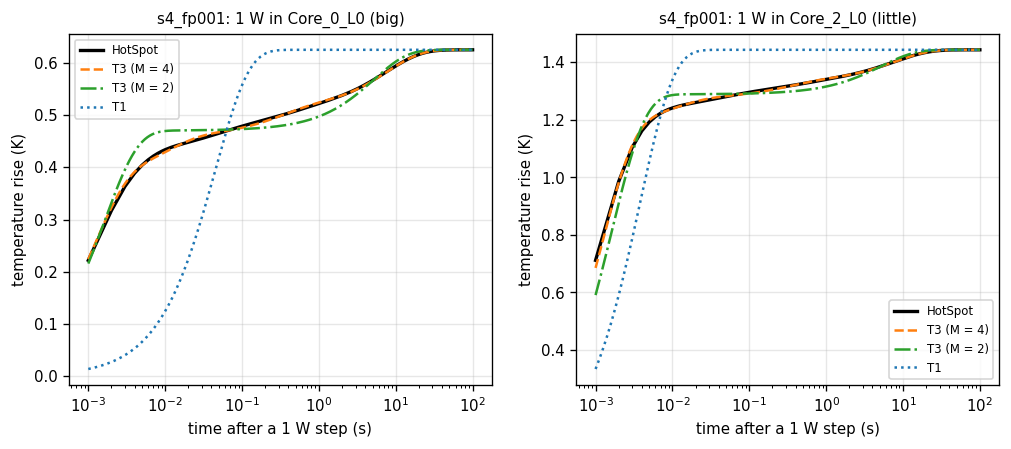
\includegraphics[width=0.9\linewidth]{P1-1_step_calibration/results/step_response_fits_stage3.png}
  \caption{Step responses to 1\,W in a big core (left) and a little core (right), log time axis.}
  \label{fig:steps}
\end{figure}

\subsection{Following HotSpot over time}\label{sec:follow}
Tested from a cold chip on a 2\,s trace on each of the 24 floorplans, plus longer 10\,s
traces.

\begin{center}
\small
\begin{tabular}{@{}l c c c c@{}}
\toprule
Model & Mean error & Worst error & Time per step & Size \\
\midrule
T1 & 7.25\,K & 14.6\,K & 1.5\us & 1.0\,kB \\
T3, $M=2$ & 0.92\,K & 2.9\,K & 3.0\us & 1.9\,kB \\
T3, $M=3$ & 0.19\,K & 1.1\,K & 3.0\us & 2.8\,kB \\
T3, $M=4$ & 0.090\,K & 0.30\,K & 3.1\us & 3.7\,kB \\
T3, $M=6$ & 0.0093\,K & 0.13\,K & 3.2\us & 5.6\,kB \\
T2 ARX(2,2) & 0.19\,K & 0.57\,K & 5.4\us & 6.2\,kB \\
\bottomrule
\end{tabular}
\end{center}
Increasing $M$ improves accuracy at the cost of model size; the time per step stays the same.

\begin{figure}[H]
  \centering
  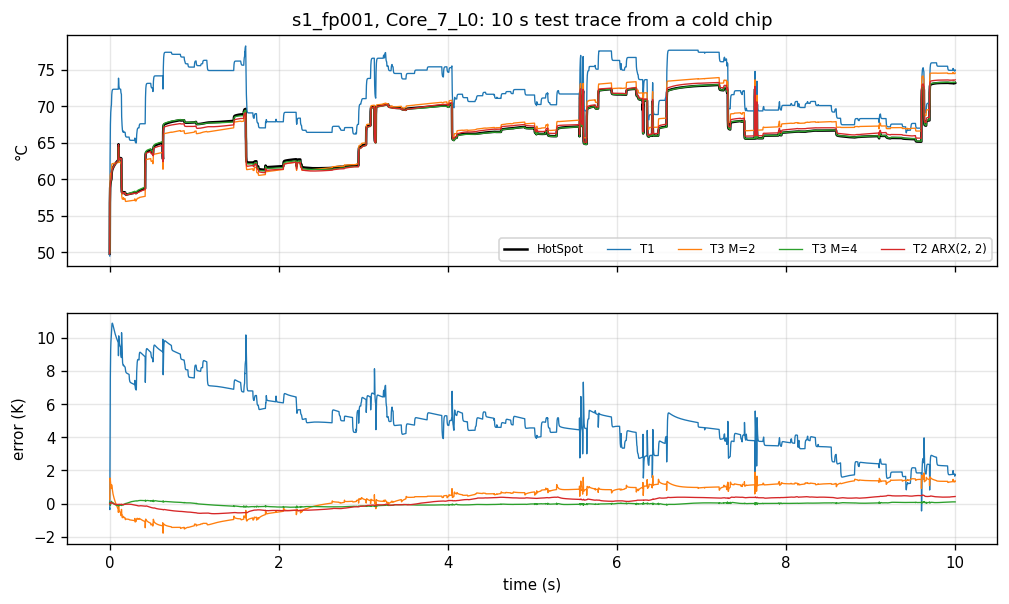
\includegraphics[width=0.75\linewidth]{P3-1_transient_predictor/results/trace_example.png}
  \caption{HotSpot and the models on one 10\,s test trace from a cold chip (top) and their error
  (bottom); T3 sits on top of HotSpot.}
  \label{fig:trace}
\end{figure}

\subsection{Trade-offs}
Figure~\ref{fig:pareto} collects every model's size, worst error and speed, using the 10\,s traces
for the transient models. Among the transient models, T3 alone forms the Pareto front from $M = 4$
on (0.31\,K worst error on these traces, and below). At 2--3\,kB, ARX is on the front
next to T3 with $M = 2$--3, but all of these are about 1--3\,K off at worst. In steady state there
is no trade-off: S1 is exact already at 464\,B (32-bit numbers), and every smaller model (the
compressed S2 variants of Stage 2) has a worst error of 3--12\,K.

\begin{figure}[H]
  \centering
  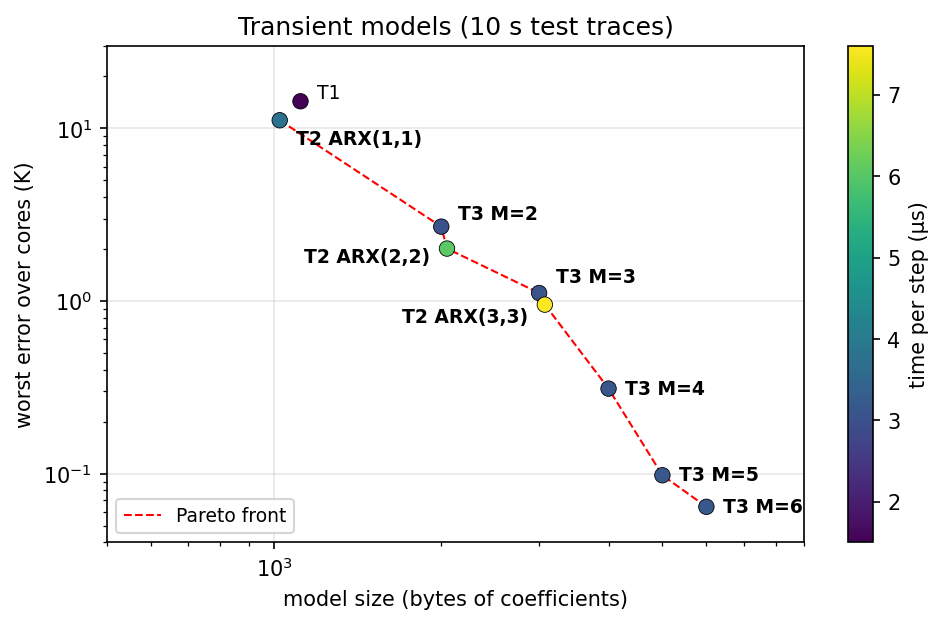
\includegraphics[width=0.68\linewidth]{P3-3_pareto/results/pareto_transient_report.png}\\[4pt]
  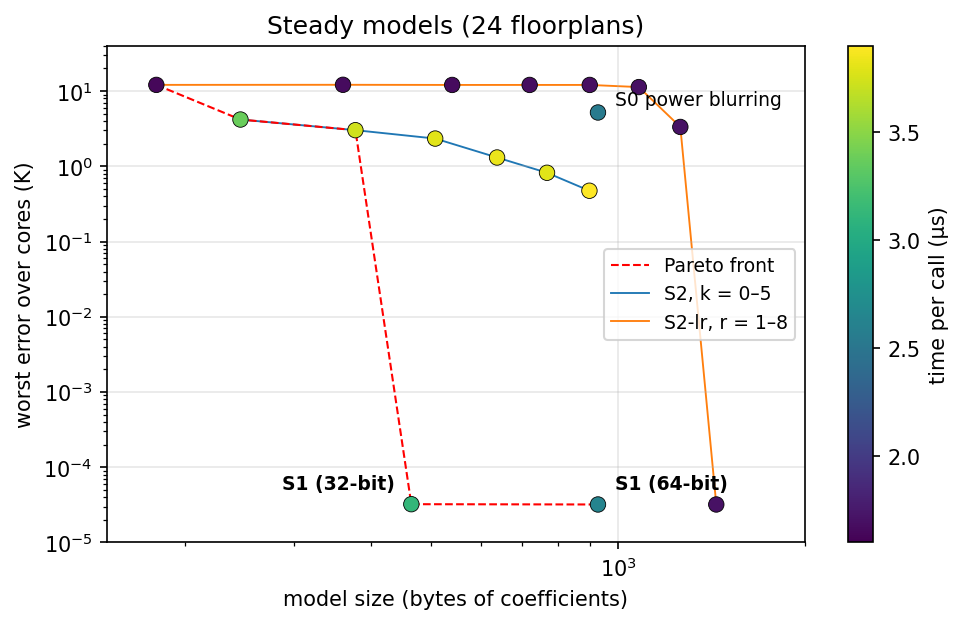
\includegraphics[width=0.68\linewidth]{P3-3_pareto/results/pareto_steady_report.png}
  \caption{Model size against worst error for the transient (top) and steady (bottom) models;
  colour is the prediction time. Bold labels and the red dashed line: the Pareto front (no other
  model is both smaller and more accurate).}
  \label{fig:pareto}
\end{figure}

%=====================================================================
\section{The final transient model}

\subsection{T3 with four time constants}
The transient model is T3 with $M=4$ (Equation~\eqref{eq:t3}). Of the three families (T1, ARX
and T3), we chose it because:
\begin{itemize}
  \item it meets the targets with room to spare: 0.09\,K mean and 0.30\,K worst error against
        0.5\,K and 1\,K, at 3.1\us\ per step and 3.7\,kB;
  \item it is exact in steady state;
  \item it gives the best accuracy per byte, and $M$ is one knob for more accuracy ($M=6$: 0.13\,K
        worst for 5.6\,kB).
\end{itemize}
T1 was ruled out because one time constant cannot cover 1\,ms to 8\,s (14\,K worst), and ARX
because it is about 2$\times$ less accurate (0.19\,K mean and 0.57\,K worst error) and needs a long
recorded trace.

\subsection{Testing on 52 generated floorplans}\label{sec:gen}
The models were developed and evaluated on the 24 floorplans of the main set. For confirmation, we
tested them on 52 floorplans they had never seen:
\begin{itemize}
  \item \textbf{Floorplans.} Our generator produced 13 floorplans in each of the four given styles,
        with the same cores (2 big, 6 little), the same file format and layer stack, and placement
        rules that imitate each style.
  \item \textbf{Tests.} T3 on a 2\,s trace from a cold chip, in which every core switches
        between power levels in phases of 1\,ms to 2\,s.
\end{itemize}

\begin{center}
\small
\begin{tabular}{@{}l c c c@{}}
\toprule
Style & Floorplans & T3 mean & T3 worst \\
\midrule
Style 1 & 13 & 0.108\,K & 0.34\,K \\
Style 2 & 13 & 0.114\,K & 0.32\,K \\
Style 3 & 13 & 0.085\,K & 0.31\,K \\
Style 4 & 13 & 0.056\,K & 0.26\,K \\
All generated & 52 & 0.091\,K & 0.34\,K \\
Main set & 24 & 0.090\,K & 0.30\,K \\
\bottomrule
\end{tabular}
\end{center}

\textbf{The results carry over.} Over 52 new floorplans T3 is off by 0.09\,K on average, the same as
on the main set.

\begin{figure}[H]
  \centering
  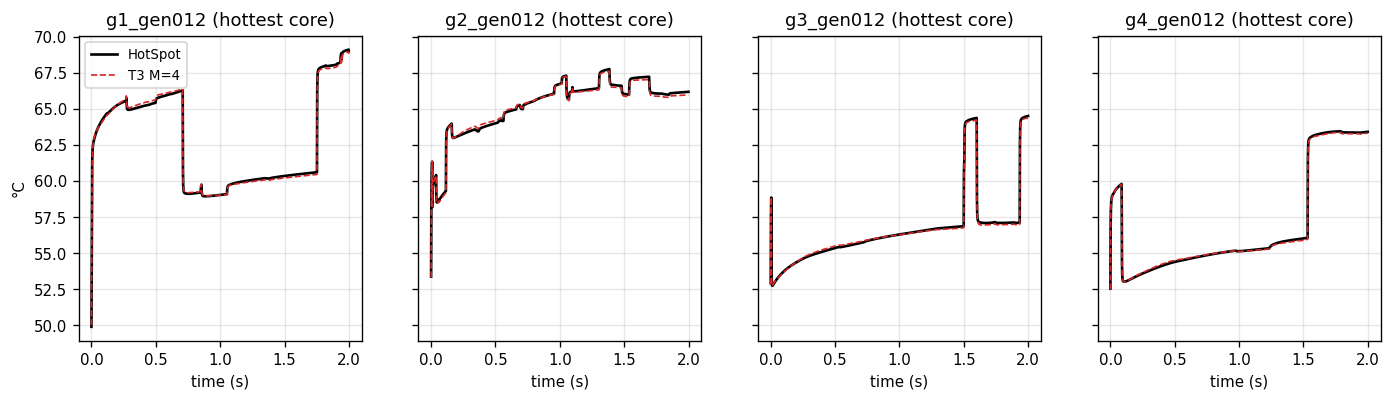
\includegraphics[width=\linewidth]{extended_validation/results/transient_check.png}
  \caption{The hottest core of one generated floorplan per style on its 2\,s test trace; T3 (red
  dashed) follows HotSpot (black).}
  \label{fig:gen}
\end{figure}

\begin{figure}[H]
  \centering
  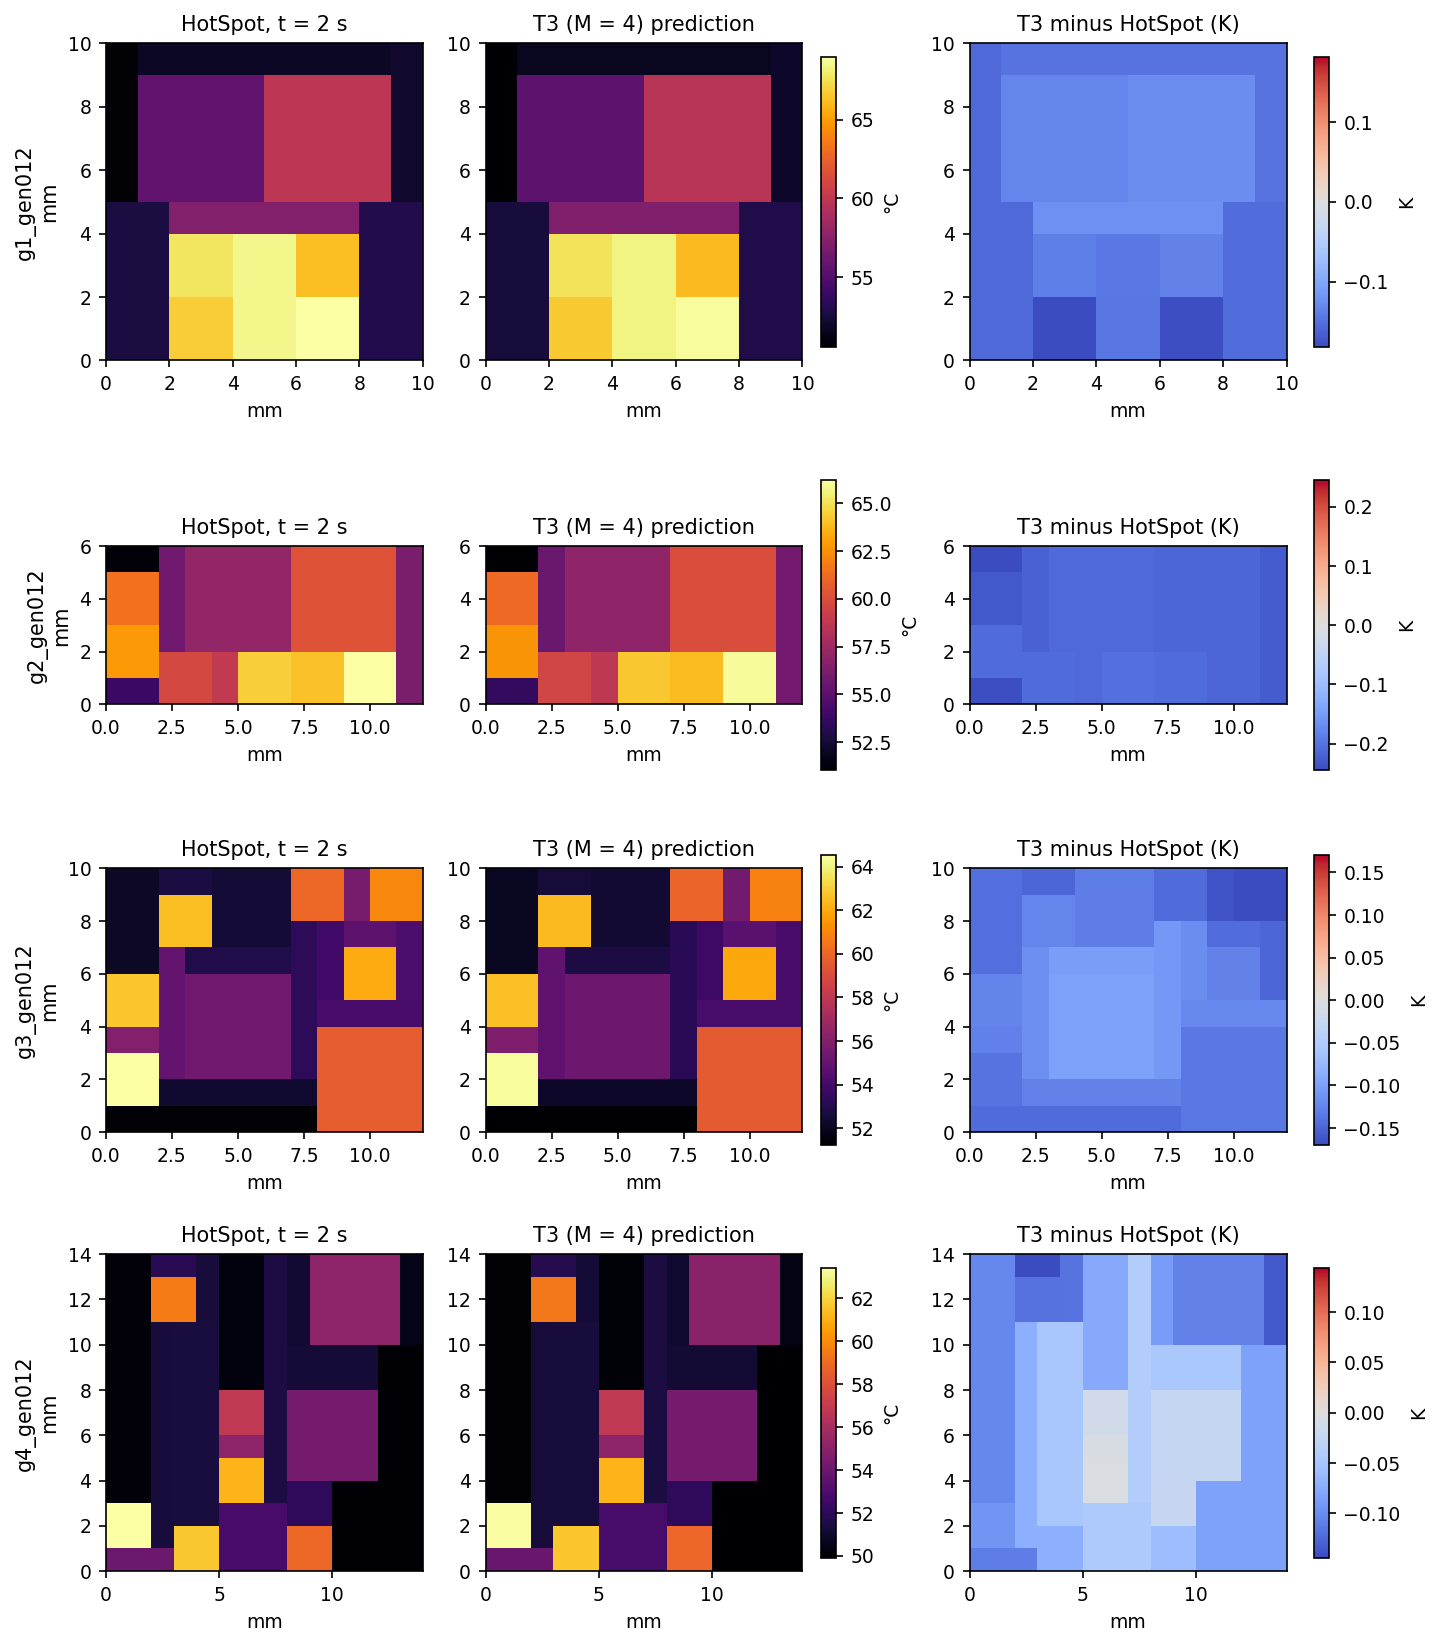
\includegraphics[width=0.66\linewidth]{extended_validation/results/heatmaps_t3_report.png}
  \caption{T3 at the end of the 2\,s test trace, one generated floorplan per style. Columns:
  HotSpot's block temperatures; T3's prediction (same colour scale); T3 minus HotSpot in kelvin.}
  \label{fig:maps}
\end{figure}

%=====================================================================
\section{Robustness}

\subsection{Unusual inputs}
The first row is the normal trace, for reference.
\begin{center}
\small
\begin{tabular}{@{}l c c@{}}
\toprule
Case & T3 mean & T3 worst \\
\midrule
Normal trace (reference) & 0.10\,K & 0.32\,K \\
Steady power at 3$\times$ the maximum (S1) & 0.00002\,K & 0.00005\,K \\
Transient at 2$\times$ power & 0.21\,K & 0.64\,K \\
Bursty power, switching every 1--5\,ms & 0.11\,K & 0.44\,K \\
Warm start (after the first 50\,ms)$^{a}$ & 0.029\,K & 0.27\,K \\
\bottomrule
\end{tabular}

\smallskip
\begin{minipage}{0.9\linewidth}\footnotesize
$^{a}$ HotSpot and T3 both start from the steady state of the first power value instead of a cold
chip. The worst error is counted after the first 50 steps (50\,ms); over the very first steps it is
2.0\,K.
\end{minipage}
\end{center}
The coefficients are properties of the chip, so power levels, bursty power and the starting state
do not change the error much; every case stays within the 1\,K target.

\subsection{Changing the cooling or the ambient temperature}
The coefficients belong to one floorplan \emph{and} one package (the cooling). We changed one thing at a time (ambient 35\degC\ instead of 45\degC, or the heat-sink
convection resistance doubled from 0.1 to 0.2\,K/W or halved to 0.05\,K/W) and compared the old
models (S1 and T3, $M=4$) with models recalibrated under the new setup, on 50 random steady power
vectors and a 3\,s trace from a cold chip.

\begin{center}
\small
\begin{tabular}{@{}l l c c@{}}
\toprule
Change & Model & Steady worst & Transient worst (3\,s) \\
\midrule
Ambient 35\degC & old model, old $T_\text{amb}$ & 10.0\,K & 10.2\,K \\
 & old model, new $T_\text{amb}$ & 0.00001--0.00002\,K & 0.23--0.27\,K \\
 & recalibrated & 0.00001--0.00002\,K & 0.23--0.27\,K \\
\midrule
Convection resistance $\times 2$ & old model & 8.5\,K & 0.43--0.48\,K \\
 & recalibrated & 0.00001--0.00002\,K & 0.26--0.29\,K \\
\midrule
Convection resistance $\times 0.5$ & old model & 4.4\,K & 0.42--0.48\,K \\
 & recalibrated & 0.00002\,K & 0.20--0.22\,K \\
\bottomrule
\end{tabular}
\end{center}
A new ambient needs no recalibration: the models predict the rise above ambient, so only
$T_\text{amb}$ has to be updated (forgetting it costs 10\,K). A new heat sink does: the old
coefficients are 8.5\,K off in steady state when the convection resistance doubles and 4.4\,K when
it halves, and recalibrating restores the accuracy.

\subsection{Leakage}
Real chips leak more power when hot, which breaks linearity. Leakage current grows roughly
exponentially with temperature~\cite{liao05}. HotSpot has a built-in leakage model (its function
\texttt{calc\_leakage}, steady state only~\cite{hotspot6}) in which every block of the silicon
layer, white space included, leaks
\begin{equation}
  P_{\text{leak},i}(T_i) = \alpha\, A_i\, e^{\beta\,(T_i - 383.15\,\text{K})},
  \qquad \alpha = 1.5\times10^{4}\,\text{W/m}^2,\ \beta = 0.036\,\text{K}^{-1},
  \label{eq:leak}
\end{equation}
where $A_i$ is the block's area and $\alpha$, $\beta$ are HotSpot's default values, so leakage
doubles about every 19\,K. HotSpot iterates power and temperature until they settle. Test: 50
random power vectors per floorplan.

\textbf{The fix to S1.} The chip is still linear in the \emph{total} power, so the calibrated
coefficients stay valid; only the leakage has to be added as extra power. Starting from the plain S1 prediction $T^{(0)} = T_\text{amb} + G\,P$, the loop repeats
\begin{equation}
  T^{(k+1)} = T_\text{amb} + G\left(P + P_\text{leak}\big(T^{(k)}\big)\right)
  \label{eq:leakloop}
\end{equation}
until the temperatures change by less than $10^{-4}$\,K.

\textbf{Result.} The chips leak 0.2--0.5\,W. Ignoring leakage (S1 alone) costs 0.08--0.10\,K at
worst. The loop removes this error, down to HotSpot's output precision ($1$--$2\times10^{-5}$\,K),
in 3 iterations and 22--25\us: about 10$\times$ slower than S1 alone but still about
10{,}000$\times$ faster than one HotSpot run. HotSpot does not support leakage in transient runs,
so the transient side could not be tested.

%=====================================================================
\section{What went as planned, and what deviated}
\textbf{As planned:} the two-stage design; HotSpot as the reference, patched to print 6 decimals so
that errors of $10^{-5}$\,K can be measured; S1 as the steady model; T3 as the transient model;
evaluation on accuracy, time and size; the calibration-is-needed check; robustness studies. All
accuracy, speed and size targets were met.

\textbf{What deviated:}
\begin{itemize}
  \item \textbf{Dataset.} Besides the 23 given floorplans (plus HET-A) we planned to use, we
        generated 52 synthetic floorplans in the same styles, to test on layouts the models had
        never seen.
  \item \textbf{Hot spots.} Instead of one hottest cell per core, S1-hot-max covers every cell of a
        core and drops cells that can never be the hottest; it is exact and still small.
\end{itemize}

%=====================================================================
\section{Pending items (for Stage 4)}
\begin{itemize}
  \item The \texttt{ltp} tool: calibrate, steady and transient prediction, and a benchmark against
        HotSpot.
  \item Final report, code archive, README with run instructions, and presentation feedback.
\end{itemize}

%=====================================================================
\section{Future scope}
\begin{itemize}
  \item Thermal management: run S1 and T3 inside a controller that throttles or migrates tasks
        before a core overheats.
  \item Leakage in transient prediction, with a simulator that supports it.
\end{itemize}

%=====================================================================
\section{LLM assistance disclosure}
LLMs were used to understand HotSpot, for literature review to select appropriate models, generate
floorplans, and calibration and testing scripts.

\begin{thebibliography}{99}\small
\setlength{\itemsep}{0pt}
\bibitem{hotspot} W.~Huang, S.~Ghosh, S.~Velusamy, K.~Sankaranarayanan, K.~Skadron and
  M.~R. Stan, ``HotSpot: A Compact Thermal Modeling Methodology for Early-Stage VLSI Design,''
  \emph{IEEE TVLSI} 14(5):501--513, 2006.
\bibitem{hotspot6} R.~Zhang, M.~R. Stan and K.~Skadron, ``HotSpot 6.0: Validation, Acceleration
  and Extension,'' Univ. of Virginia, Tech. Rep. CS-2015-04, 2015.
\bibitem{liao05} W.~Liao, L.~He and K.~M. Lepak, ``Temperature and Supply Voltage Aware
  Performance and Power Modeling at Microarchitecture Level,'' \emph{IEEE TCAD} 24(7):1042--1053,
  2005.
\bibitem{coskun09} A.~K. Coskun, T.~S. Rosing and K.~C. Gross, ``Utilizing Predictors for
  Efficient Thermal Management in Multiprocessor SoCs,'' \emph{IEEE TCAD} 28(10), 2009.
\bibitem{singla15} G.~Singla, G.~Kaur, A.~K. Unver and U.~Y. Ogras, ``Predictive Dynamic Thermal
  and Power Management for Heterogeneous Mobile Platforms,'' in \emph{Proc. DATE}, 2015.
\end{thebibliography}

\end{document}
